\documentclass[letterpaper, 11pt]{extarticle}
% \usepackage{fontspec}

% ==================================================

% document parameters
% \usepackage[spanish, mexico, es-lcroman]{babel}
\usepackage[english]{babel}
\usepackage[margin = 1in]{geometry}

% ==================================================

% Packages for math
\usepackage{mathrsfs}
\usepackage{tikz}
\usepackage{amsfonts}
\usepackage{amsmath}
\usepackage{amsthm}
\usepackage{amssymb}
\usepackage{physics}
\usepackage{dsfont}
\usepackage{esint}

% ==================================================

% Packages for writing
\usepackage{enumerate}
\usepackage[shortlabels]{enumitem}
\usepackage{framed}
\usepackage{csquotes}

% ==================================================

% Miscellaneous packages
\usepackage{float}
\usepackage{tabularx}
\usepackage{xcolor}
\usepackage{multicol}
\usepackage{subcaption}
\usepackage{caption}
\captionsetup{format = hang, margin = 10pt, font = small, labelfont = bf}

% Citation
\usepackage[round, authoryear]{natbib}

% Hyperlinks setup
\usepackage{hyperref}
\definecolor{links}{rgb}{0.36,0.54,0.66}
\hypersetup{
   colorlinks = true,
    linkcolor = black,
     urlcolor = blue,
    citecolor = blue,
    filecolor = blue,
    pdfauthor = {Author},
     pdftitle = {Title},
   pdfsubject = {subject},
  pdfkeywords = {one, two},
  pdfproducer = {LaTeX},
   pdfcreator = {pdfLaTeX},
   }
\usepackage{titlesec}
\usepackage[many]{tcolorbox}

% Adjust spacing after the chapter title
\titlespacing*{\chapter}{0cm}{-2.0cm}{0.50cm}
\titlespacing*{\section}{0cm}{0.50cm}{0.25cm}

% Indent 
\setlength{\parindent}{0pt}
\setlength{\parskip}{1ex}

% --- Theorems, lemma, corollary, postulate, definition ---
% \numberwithin{equation}{section}

\newtcbtheorem[]{problem}{Exercício}%
    {enhanced,
    colback = black!5, %white,
    colbacktitle = black!5,
    coltitle = black,
    boxrule = 0pt,
    frame hidden,
    borderline west = {0.5mm}{0.0mm}{black},
    fonttitle = \bfseries\sffamily,
    breakable,
    before skip = 3ex,
    after skip = 3ex
}{problem}


\newtcbtheorem[]{solution}{Resolução do Exercício}%
    {enhanced,
    colback = black!5, %white,
    colbacktitle = black!5,
    coltitle = black,
    boxrule = 0pt,
    frame hidden,
    borderline west = {0.5mm}{0.0mm}{black},
    fonttitle = \bfseries\sffamily,
    breakable,
    before skip = 3ex,
    after skip = 3ex
}{solution}

\tcbuselibrary{skins, breakable}

% --- You can define your own color box. Just copy the previous \newtcbtheorm definition and use the colors of yout liking and the title you want to use.
% --- Basic commands ---
%   Euler's constant
\newcommand{\eu}{\mathrm{e}}

%   Imaginary unit
\newcommand{\im}{\mathrm{i}}

%   Sexagesimal degree symbol
\newcommand{\grado}{\,^{\circ}}

% --- Comandos para álgebra lineal ---
% Matrix transpose
\newcommand{\transpose}[1]{{#1}^{\mathsf{T}}}

%%% Comandos para cálculo
%   Definite integral from -\infty to +\infty
\newcommand{\Int}{\int\limits_{-\infty}^{\infty}}

%   Indefinite integral
\newcommand{\rint}[2]{\int{#1}\dd{#2}}

%  Definite integral
\newcommand{\Rint}[4]{\int\limits_{#1}^{#2}{#3}\dd{#4}}

%   Dot product symbol (use the command \bigcdot)
\makeatletter
\newcommand*\bigcdot{\mathpalette\bigcdot@{.5}}
\newcommand*\bigcdot@[2]{\mathbin{\vcenter{\hbox{\scalebox{#2}{$\m@th#1\bullet$}}}}}
\makeatother

%   Hamiltonian
\newcommand{\Ham}{\hat{\mathcal{H}}}

%   Trace
\renewcommand{\Tr}{\mathrm{Tr}}

% Christoffel symbol of the second kind
\newcommand{\christoffelsecond}[4]{\dfrac{1}{2}g^{#3 #4}(\partial_{#1} g_{#2 #4} + \partial_{#2} g_{#1 #4} - \partial_{#4} g_{#1 #2})}

% Riemann curvature tensor
\newcommand{\riemanncurvature}[5]{\partial_{#3} \Gamma_{#4 #2}^{#1} - \partial_{#4} \Gamma_{#3 #2}^{#1} + \Gamma_{#3 #5}^{#1} \Gamma_{#4 #2}^{#5} - \Gamma_{#4 #5}^{#1} \Gamma_{#3 #2}^{#5}}

% Covariant Riemann curvature tensor
\newcommand{\covariantriemanncurvature}[5]{g_{#1 #5} R^{#5}{}_{#2 #3 #4}}

% Ricci tensor
\newcommand{\riccitensor}[5]{g_{#1 #5} R^{#5}{}_{#2 #3 #4}}

\begin{document}

\begin{Large}
    \textsf{\textbf{Lista de Revisão 01 - Linguagens Formais e Autômatos}}
    
    Ciência da Computação - Universidade Cruzeiro do Sul Campus Guarulhos
\end{Large}

\vspace{1ex}

\textsf{\textbf{Estudante:}} \text{Gabriel Morishita}, \href{mailto:your.email@hotmail.com}{\texttt{gabriel.zanferrari@cs.cruzeirodosul.edu.br}}\\
\textsf{\textbf{Professor:}} \text{Sergio Ricardo Master Penedo}, \href{mailto:teacher.email@hotmail.com}{\texttt{spenedo@pf.cruzeirodosul.edu.br}}


\vspace{2ex}

\begin{problem}{}{}
Sabendo que \{A={1, 2, 3, 4}\}, \{B={4, 5, 6}\} e \{C={1, 6, 7, 8, 9}\}. Qual o conjunto (A$\cap$B)$\cup$C
\end{problem}

\begin{solution}{}{}
    Podemos representar o conjunto (A$\cap$B)$\cup$C como:
    
    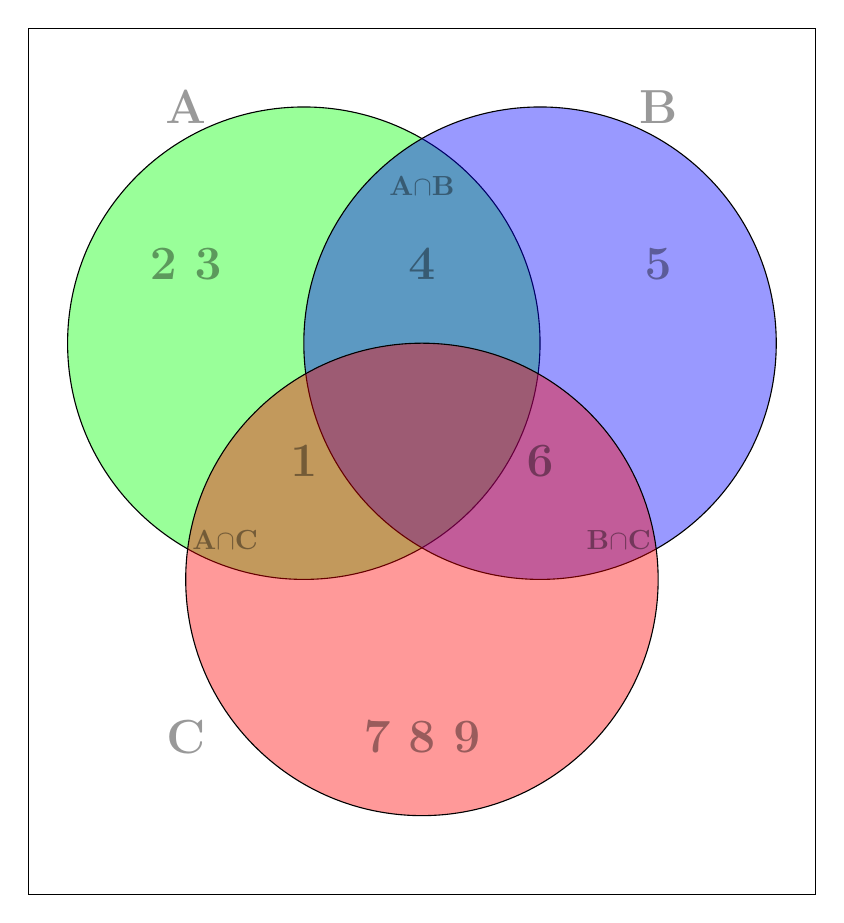
\begin{tikzpicture}
	\begin{scope} [fill opacity = .4]
    \draw (-5,5) rectangle (5,-6);
    \draw[fill=green, draw = black] (-1.5,1) circle (3);
    \draw[fill=blue, draw = black] (1.5,1) circle (3);
    \draw[fill=red, draw = black] (0,-2) circle (3);

    \node at (-3,4) {\LARGE\textbf{A}};
    \node at (-3,2) {\LARGE\textbf{2 3}};

    \node at(0,3) {\textbf{A$\cap$B}};
    \node at(0,2) {\LARGE\textbf{4}};
    
    \node at(-2.5,-1.5) {\textbf{A$\cap$C}};
    \node at(-1.5,-0.5) {\LARGE\textbf{1}};
    
    \node at (3,4) {\LARGE\textbf{B}};
    \node at (3,2) {\LARGE\textbf{5}};

    \node at(2.5,-1.5) {\textbf{B$\cap$C}};
    \node at(1.5,-0.5) {\LARGE\textbf{6}};
    
    \node at (-3,-4) {\LARGE\textbf{C}};
    \node at (0,-4) {\LARGE\textbf{7 8 9}};
    
    % \draw[help lines](-5,5) grid (5,-6);    This line can draw the grid lines to help guide you. I use these when I'm writing the code and then delete this line when I publish the pdf.    
    \end{scope}
    \end{tikzpicture}
    
    Com isso, tomamos que A$\cap$B$\cap$C=$\varnothing$. \\
    Portanto, para solucionar basta pegarmos o conjunto A$\cap$B=\{{4}\} e somar com tudo que há em C, obtendo o resultado (A$\cap$B)$\cup$C=\{{1, 4, 6, 7, 8, 9}\}

    \textbf{Resposta final: (A$\cap$B)$\cup$C=\{{1, 4, 6, 7, 8, 9}\}}
\end{solution}

\newpage

\begin{problem}{}{}
José Carlos e Marlene são os pais de Valéria. A família quer viajar nas férias de julho. José Carlos
conseguiu tirar suas férias na fábrica do dia 2 ao dia 28. Marlene obteve licença no escritório de 5 a
30. As férias de Valéria na escola vão de 1 a 25. Durante quantos dias a família poderá viajar sem
faltar as suas obrigações?
\end{problem}

\begin{solution}{}{}

    Para resolver esse exercício, primeiro montemos uma linha do tempo com a disponibilidade de cada membro da família. \\
    José Carlos: dias 2 $\rightarrow$ 28, representado pela cor \colorbox{green}{verde} \\
    Marlene: dias 5 $\rightarrow$ 30, representada pela cor \colorbox{red}{vermelha}\\
    Valéria: dias 1 $\rightarrow$ 25, representada pela cor \colorbox{orange}{laranja}\\
    
    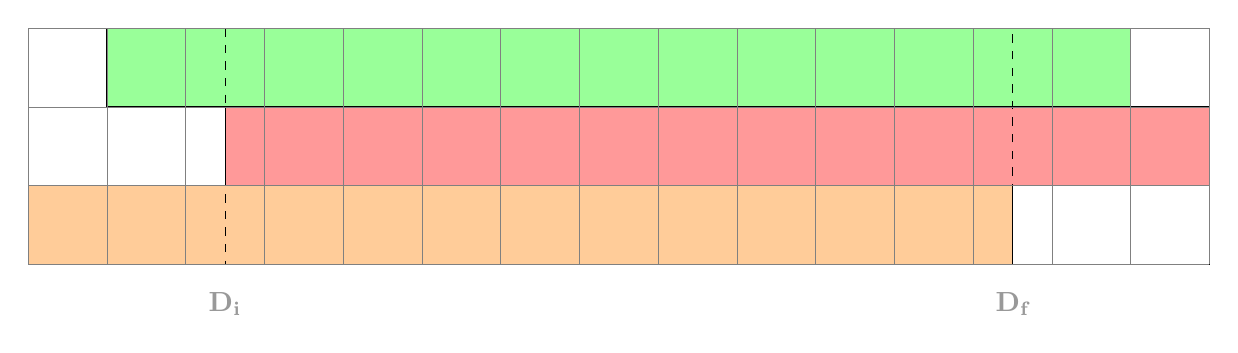
\begin{tikzpicture}
	\begin{scope} [fill opacity = .4]
    \draw (0,3) rectangle (15,0);

    \draw[fill=green, draw = black] (1,3) rectangle (14, 2); % José Carlos
    \draw[fill=red, draw = black] (2.5,2) rectangle (15, 1); % Marlene
    \draw[fill=orange, draw = black] (0,1) rectangle (12.5, 0); % Valeria

    \draw[draw = black, dashed] (2.5,3) rectangle (12.5, 0);

    \node at (2.5, -0.5) {\textbf{D\textsubscript{i}}};
    \node at (12.5, -0.5) {\textbf{D\textsubscript{f}}};
    
    \draw[help lines](0,3) grid (15,0);       
    \end{scope}
    \end{tikzpicture}\\
    \textit{Nota: Cada dia é representado por 1/2 quadrado}\\

    Para obter o resultado, precisamos demarcar um período, dado pela maior data de início e pela menor data limite. Podemos chamar esses termos respectivamente de D\textsubscript{i} e D\textsubscript{f}. \\
    Podemos definir dois conjuntos, o conjunto D\textsubscript{i} dado por \{{2, 5, 1}\} e o conjunto D\textsubscript{f} dado por \{{28, 30, 25}\}. \\
    Com estes conjuntos, basta procurar pelo maior termo do primeiro conjunto e uni-lo ao menor termo do segundo, obtendo assim o período \{{5, 25}\}. O mesmo período pode ser visto no gráfico ao traçarmos linhas imaginárias nos pontos respectivos, tendo assim uma representação do período de férias ideal para solução do problema.

    \textbf{Resposta final: $\xrightarrow[D\textsubscript{i}D\textsubscript{f}]{}$=\{{5, 25}\}}
\end{solution}

\begin{problem}{}{}
Em uma classe de 30 alunos, 16 gostam de Matemática e 20 gostam de História. Qual o número
de alunos desta classe que gostam de Matemática e História?
\end{problem}

\begin{solution}{}{}
    Vamos representar essa turma como sendo, \\ 
        $\bullet$ A = Pessoas que gostam de Matemática. \\
        $\bullet$ B = Pessoas que gostam de História.   \\

    Dessa maneira, podemos representar o seguinte diagrama de venn: \\
    
    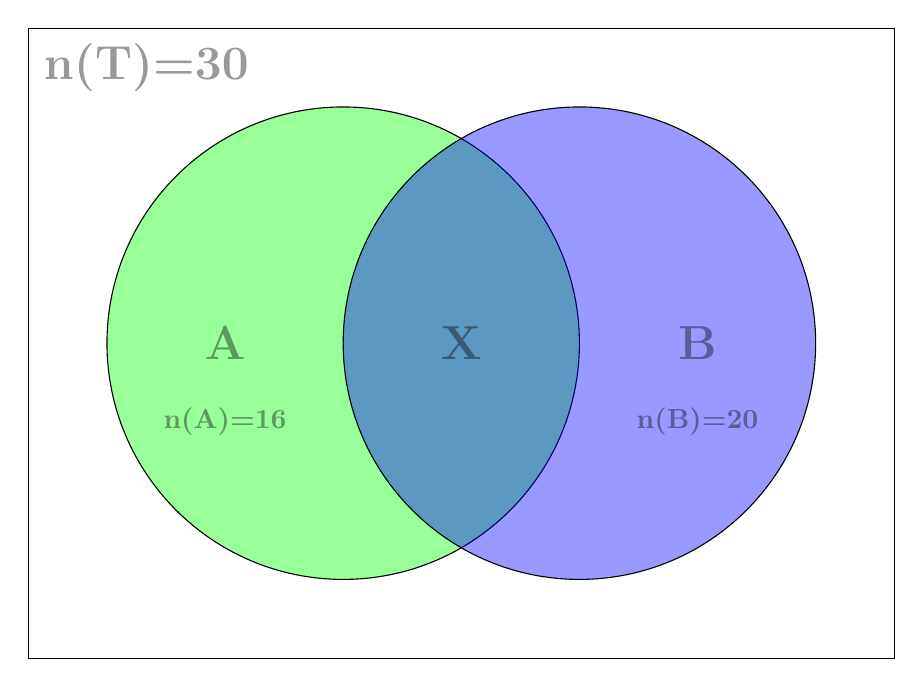
\begin{tikzpicture}
	\begin{scope} [fill opacity = .4]
    \draw (0,8) rectangle (11,0);

    \draw[fill=green, draw = black] (4,4) circle (3);
    \draw[fill=blue, draw = black] (7,4) circle (3);
    \node at (1.5,7.5) {\LARGE\textbf{n(T)=30}};

    \node at (2.5,4) {\LARGE\textbf{A}};
    \node at (2.5,3) {\textbf{n(A)=16}};

    \node at (8.5,4) {\LARGE\textbf{B}};
    \node at (8.5,3) {\textbf{n(B)=20}};
    
    \node at (5.5,4) {\LARGE\textbf{X}};
    
    % \draw[help lines](-5,5) grid (5,-6);    This line can draw the grid lines to help guide you. I use these when I'm writing the code and then delete this line when I publish the pdf.    
    \end{scope}
    \end{tikzpicture}

    Podemos levar como regra de que A'$\cap$B'=(A$\cup$B)'=$\varnothing$, e de que a função n(X) retorna como produto a quantidade de itens em X.
    Analisando então o diagrama, podemos também concluir de que, se o total de alunos n(T) é 30, e é evidente de que n(A$\cup$B)$>$30. \\

    Como não temos um número para trabalhar, também declaramos A$\cap$B como sendo X. \\
    Dito isso, podemos criar a regra $n(A\cup B) \equiv 30$. Ou seja, a soma das quantias de A e B devem ser exatamente 30. \\
    
    Com isso, podemos dizer que $n(A) + X + n(B) \equiv 30$, que se traduz para $16 + X + 20 \equiv 30$. \\
    Resolvendo a equação de primeiro grau, temos que \\ $X \equiv 30 - (16 + 20) \Rightarrow X = 30-26$ \textbf{$\therefore$ X = -6} \\

    Como não é possível que a interseção entre dois conjuntos seja negativa, podemos interpretar da seguinte maneira:
    
        \[\mid X\mid = (n(A) + n(B)) - n(T)\]

    Podemos então concluir que, o número mínimo de alunos que podem gostar de ambas as matérias é 6, porém, 6 não é a única resposta. \\ 
    O número 6 indica a quantidade mínima contida em X, porém a quantidade máxima ainda não foi definida.

    Podemos então, assumir que a resposta é um conjunto que contém o menor número possível (6) e o maior número possível (iremos chamar de Y por agora).\\
    Para descobrir o maior valor, podemos assumir que
        \[Y = n(C\textsubscript{1}) < n(C\textsubscript{2}) < ... <   \frac{n(C\textsubscript{N})}{N\rightarrow \infty} \]
    Onde Y é a quantidade máxima de itens possível em um conjunto.\\ 
    Iremos chamá-la de "Fórmula de quantidade máxima de itens em um conjunto". \\
    A expressão acima pode ser traduzida como, Y é igual a quantidade de itens do conjunto 1, que deve ser menor do que a quantidade de itens do conjunto 2, e menor do que qualquer outro conjunto subsequente. Ou seja, Y só pode ser igual a quantidade de itens do menor conjunto analisado. \\

    \textbf{Resposta final: O conjunto de respostas possíveis é $\{{n \in \mathbb{R} \mid 6 \leq n \leq 16}\}$}
    
    
\end{solution}

\begin{problem}{}{}   
    Sejam os conjuntos A com 2 elementos, B com 3 elementos e C com 4 elementos, então
    pode-se afirmar que:
    \begin{enumerate}[(a)]
        \item $A\cap B$ tem no máximo 1 elemento
        \item $A \cup C$ tem no máximo 5 elementos
        \item $(A \cap B) \cap C$ tem no máximo 2 elementos
        \item $(A \cup B) \cap C$ tem no máximo 2 elementos
        \item $(A \cap \varnothing)$ tem pelo menos dois elementos
    \end{enumerate}
\end{problem}

\begin{solution}{}{}
    Vamos utilizar como método de solução a tentativa e erro. \\
    Porém, iremos tomar como regras: \\
    $\bullet$ A função n(X) retorna como produto a quantidade de itens em X. \\ 
    $\bullet$ A função max(f(x)) retorna como produto a quantidade máxima de itens oriunda de uma função de X, que pode ser interpretada como uma função genérica e pode ser substituída por qualquer expressão entre um ou mais conjuntos.  \\
    $\bullet$ A função min(f(x) retorna como produto a quantidade mínima de itens oriunda de uma função de X, que pode ser interpretada como uma função genérica e pode ser substituída por qualquer expressão entre um ou mais conjuntos. \\
    \begin{enumerate}[(a)]
        \item Essa afirmativa pode ser descartada, pois, aplicando a fórmula de quantidade máxima de itens em um conjunto,
        podemos definir a quantidade máxima entre A e B como sendo a quantidade de itens do conjunto com menos itens, que nesse caso, se traduz como 2. \\
        $\therefore max(A\cap B) \leq 2 \implies max(A\cap B) \ne 1$
        \item Essa afirmativa pode ser descartada, pois $A\cup C = 6 \Rightarrow 6 > 1 \therefore max(A\cup C) \ne 1$
        \item Essa afirmativa é a correta, mas para chegar ao resultado, iremos resolver a quantidade máxima de itens de $(A\cap B)$, ou seja, $max(A\cap B)$. \\
            \begin{enumerate}[(i)]
              \item Para $max(A\cap B)$, podemos definir, utilizando a fórmula de quantidade máxima de itens em um conjunto, que $max(A\cap B) = 2$
              \item Atribuindo $(A\cap B)$ a um conjunto D, onde $n(D)=2 \impliedby max(A\cap B) =2$, temos a afirmação do enunciado como $D\cap C$
              \item Sabendo que $n(D)=2$ e $n(C) > n(D)$, podemos afirmar que $n(D)$ é o máximo de itens que pode existir no conjunto $D\cap C$, o que é, outra maneira de afirmar que: \textbf{(A $\cap$ B) $\cap$ C tem no máximo 2 elementos}
            \end{enumerate}
    \end{enumerate}

    \textbf{Resultado final: A alternativa correta é a alternativa (c)}
\end{solution}

\begin{problem}{}{}
    Em uma pesquisa de mercado, verificou-se que 15 pessoas utilizam pelo menos um dos produtos
    A ou B. Sabendo que 10 destas pessoas não usam o produto B e que 2 destas pessoas não usam o
    produto A, qual é o número de pessoas que utilizam os produtos A e B?
\end{problem}

\begin{solution}{}{}
    Sabendo que A e B são conjuntos onde n(A) e n(B) são indefinidos. \\
    Podemos concluir, de acordo com o enunciado, que: \\
    $\bullet T = 15$ \\
    $\bullet  A\cap B'  = 10$ \\
    $\bullet A'\cap B = 2$ \\
    $\bullet A\cap B = X$ \\
    $\bullet \therefore A\cap B \impliedby (A'\cap B) + (A\cap B') - X = T$ \\
    
    Podemos então definir o problema com este diagrama:

    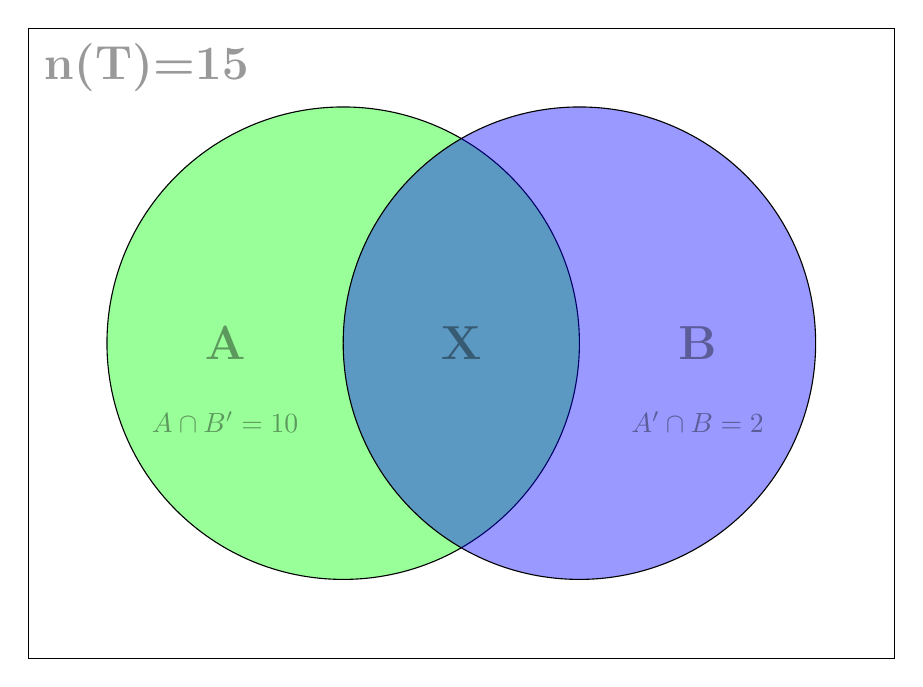
\begin{tikzpicture}
	\begin{scope} [fill opacity = .4]
        \draw (0,8) rectangle (11,0);

        \draw[fill=green, draw = black] (4,4) circle (3);
        \draw[fill=blue, draw = black] (7,4) circle (3);
        \node at (1.5,7.5) {\LARGE\textbf{n(T)=15}};
    
        \node at (2.5,4) {\LARGE\textbf{A}};
        \node at (2.5,3) {\textbf{$A\cap B'  = 10$}};
    
        \node at (8.5,4) {\LARGE\textbf{B}};
        \node at (8.5,3) {\textbf{$A'\cap B  = 2$}};
        
        \node at (5.5,4) {\LARGE\textbf{X}};
    \end{scope} 
    \end{tikzpicture}
    
    Solucionando a equação acima, temos que $X=(A'\cap B) + (A\cap B')-T$ \\
    Que é igual a $X=10+2-15 = 3 \implies X=3$ \\
    \textbf{Resposta final: 3 Pessoas.}
\end{solution}

\begin{problem}{}{}
    Em uma escola que tem 415 alunos, 221 estudam inglês, 163 estudam francês e 52 estudam
    ambas as línguas. Quantos alunos estudam inglês ou francês? Quantos alunos não estudam
    nenhuma das duas?
\end{problem}

\begin{solution}{}{}
    Tomando alunos que estudam inglês como A, e alunos que estudam francês como B, podemos definir que: \\
    $\bullet T = 415$ \\
    $\bullet  n(A)=221$ \\
    $\bullet n(B)=163$ \\
    $\bullet A\cap B = 52$ \\
    
    Podemos então definir o problema com este diagrama:

    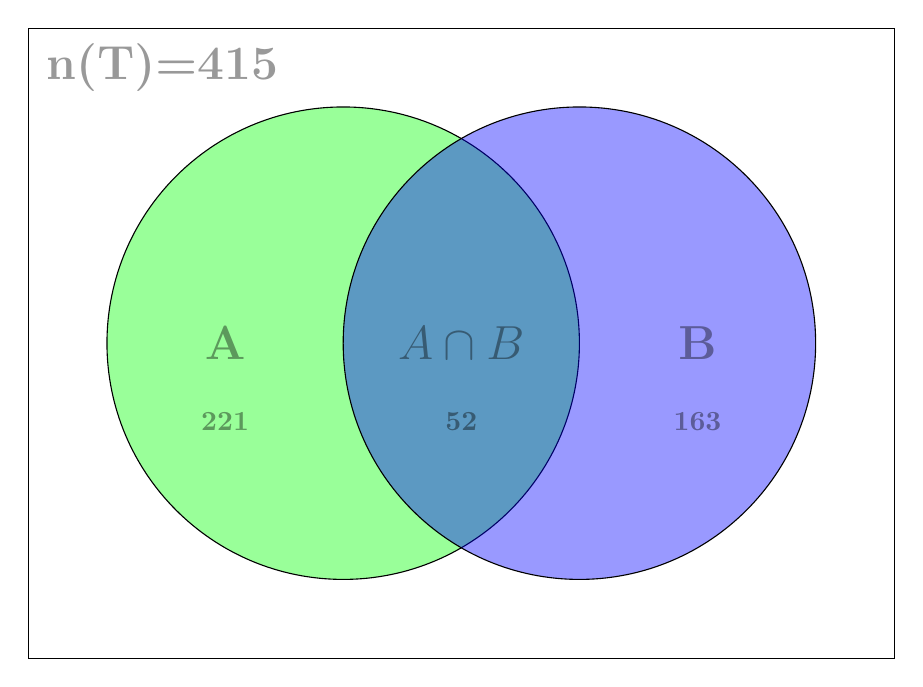
\begin{tikzpicture}
	\begin{scope} [fill opacity = .4]
        \draw (0,8) rectangle (11,0);

        \draw[fill=green, draw = black] (4,4) circle (3);
        \draw[fill=blue, draw = black] (7,4) circle (3);
        \node at (1.7,7.5) {\LARGE\textbf{n(T)=415}};
    
        \node at (2.5,4) {\LARGE\textbf{A}};
        \node at (2.5,3) {\textbf{221}};
    
        \node at (8.5,4) {\LARGE\textbf{B}};
        \node at (8.5,3) {\textbf{163}};
        
        \node at (5.5,4) {\LARGE\textbf{$A\cap B$}};
        \node at (5.5,3) {\textbf{52}};
    \end{scope} 
    \end{tikzpicture}

    Com isso, podemos definir que, a quantidade de alunos que realiza somente um tipo de aula é a quantidade total do conjunto menos a quantidade de alunos que realiza as duas aulas.
    $A\cap B' = 221 - 52$ || $A'\cap B = 163-52$ \\
    O que resulta, respectivamente, nos valores 169 e 111. Portanto, podemos definir que: $A\cup B=169+111=280$. \\
    Como o exercício quer saber a quantidade de alunos que não realiza nenhuma das duas aulas, podemos então pegar a quantidade total do conjunto (415) e subtrair a quantidade de alunos que faz alguma aula ($A\cup B$), resultando no valor 135.\\
    \textbf{Resposta final: 135 alunos não realizam nenhuma das duas aulas.}
\end{solution}

\newpage
\begin{problem}{}{}
    Determinar o conjunto X tal que:
    \begin{enumerate}[(a)]
        \item $\{{a, b, c, d}\}\cup X =\{{a, b, c, d, e}\}$
        \item $\{{c, d}\}\cup X =\{{a, c, d, e}\}$
        \item $\{{b, c, d}\}\cap X =\{{c}\}$
    \end{enumerate}
\end{problem}

\begin{solution}{}{}
    Sabemos que X é um conjunto formado por elementos desconhecidos e teremos que os encontrar.\\
    \begin{enumerate}[(a)]
        \item Podemos ver que a união entre \{a, b, c, d\} e X gera um conjunto com um elemento a mais, ou seja, podemos presumir de que $\{e\} \in X$
        \item Utilizando da mesma lógica, podemos perceber que a união entre \{a, b, c, d\} e X gera um conjunto com dois elementos a mais, ou seja, podemos presumir que $\{a, e\} \in X$
        \item Podemos, novamente, utilizar da mesma lógica, porém com a diferença de, ao invés de uma união ser uma interseção entre \{b, c, d\} e X, que nos gera um conjunto com somente um elemento \{c\}. Portanto, podemos presumir que o único termo em comum entre \{b, c, d\} e X é \{c\}, tendo assim a certeza de que $\{b, d\} \notin X$
    \end{enumerate}

    Portanto, com base nas afirmações do enunciado, podemos determinar o conjunto X como sendo \{a, c, e\}\\
    \textbf{Resposta final: $X=\{a, c, e\}$}
\end{solution}

\begin{problem}{}{}
    Um levantamento socioeconômico entre os habitantes de uma cidade revelou que, exatamente
    17\% têm casa própria; 22\% têm automóvel; 8\% têm casa própria e automóvel. Qual o percentual
    dos que não têm casa própria nem automóvel?
\end{problem}

\begin{solution}{}{}
    Para esse exercício, como estamos lidando com percentual, para facilitar a resolução vamos supor que o número total de pessoas no levantamento é 100.\\
    Também iremos associar pessoas com casa própria ao conjunto A, e pessoas com um automóvel ao conjunto B. \\
    Temos então que: \\
    $\bullet$ n(A) = 17 \\
    $\bullet$ n(B) = 22 \\
    $\bullet$ n(A$\cap$ B) = 8 \\

    Utilizando a mesma lógica do exercício 6, podemos então associar pessoas que somente possuem casa como $A\cap B' = n(A) - n(A\cap B) \implies A\cap B' = 9$. \\
    E pessoas que possuem somente carro como: $A'\cap B = n(B) - n(A\cap B) \implies A'\cap B = 14$. \\
    Como o total de habitantes (T) foi simplificado para 100, então podemos dizer que o total de habitantes que não está contido em A ou B é de $n(T) - (A\cap B') - (A\cap B) - (A'\cap B)$ \\
    que pode ser simplificado como $100-8-9-14=69$. \\
    \textbf{Resposta final: $\frac{69}{100}$ pessoas não possuem nem carro nem casa, ou, o equivalente a 69\% da pesquisa}
\end{solution}

\end{document}